  \documentclass[notheorems]{beamer}
% bibliography
\usepackage[backend=biber]{biblatex}
\bibliography{ref.bib}

\usepackage{../../template/sty/packages_math}
\usepackage{../../template/sty/packages_formatting}
\usepackage{../../template/sty/shortcuts_pm}
\usepackage{../../template/sty/beamer-template}

\graphicspath{{../expe/}}


%%%%%% Pink beamer colour theme
%% https://www.r-bloggers.com/create-your-own-beamer-template/

%%%% COLOURS

%\definecolor{CaPink}{RGB}{232, 94, 138} % default pink
%\definecolor{CaDarkUnsatPink}{RGB}{249, 26, 97} % dark unsaturated pink
%\definecolor{CaLightPink}{RGB}{253, 175, 200} % light pink
%\definecolor{CaRed}{RGB}{223, 47, 81} % red

\definecolor{CaDarker}{HTML}{C86FC9}
\definecolor{CaDark}{HTML}{E085CE}
\definecolor{CaNormal}{HTML}{F79AD3}
\definecolor{CaLight}{HTML}{F7C7DB}


%%%% THEME


\setbeamercolor{palette primary}{bg=CaDarker,fg=white}
\setbeamercolor{palette secondary}{bg=CaDark,fg=white}
\setbeamercolor{palette tertiary}{bg=CaNormal,fg=white}
\setbeamercolor{palette quaternary}{bg=CaLight,fg=white}

%% header color
% https://tex.stackexchange.com/questions/321097/how-to-change-color-of-shadow-around-frametitle-latex-beamer
\pgfdeclarehorizontalshading[frametitle.bg,frametitle right.bg]{beamer@frametitleshade}{\paperheight}{
    color(0pt)=(CaDarker);
    color(\paperwidth)=(CaDarker)}

\setbeamercolor{normal text}{fg = black}

\setbeamercolor{frametitle}{fg = white, bg = CaDarker}
\setbeamercolor{title}{fg = white, bg = CaDarker}
\setbeamercolor{subtitle}{fg = white, bg = CaDark}

\setbeamercolor{author in head/foot}{fg = white, bg = CaDarker}
\setbeamercolor{title in head/foot}{fg = white, bg = CaDarker}
\setbeamercolor{numbering in head/foot}{fg = white, bg = CaDarker}
\setbeamercolor{date in head/foot}{fg = white, bg = CaDarker}

\setbeamercolor{section in toc}{fg = CaDark}
\setbeamercolor{section in toc shaded}{fg = CaDark}

\setbeamercolor{item}{fg = CaDarker}
\setbeamercolor{subitem}{fg = CaNormal}
\setbeamercolor{subsubitem}{fg = CaLight}
\setbeamercolor{description item}{fg = CaNormal}

\setbeamercolor{bibliography entry author}{fg = CaNormal}
\setbeamercolor{bibliography entry title}{fg = black}
\setbeamercolor{bibliography entry note}{fg = CaDarker}

\setbeamercolor{footnote mark}{fg = CaDarker}

%\setbeamercolor{caption}{fg = white}
\setbeamercolor{caption name}{fg = CaDarker}
\setbeamercolor{caption source}{fg = CaDark}

% % Standard block
% \setbeamercolor{block title}{fg = white, bg = green!20!blue}
% \setbeamercolor{block body}{bg = blue!1!white}
%
% % Alert block
% \setbeamercolor{block title alerted}{fg = white, bg = red}
% \setbeamercolor{block body alerted}{bg = red!1!white}
%
% % Example block
% \setbeamercolor{block title example}{fg = white, bg = green!80!blue}
% \setbeamercolor{block body example}{bg = green!1!white}



%%%%%%% Pink beamer colour theme
%% https://www.r-bloggers.com/create-your-own-beamer-template/

%%%% COLOURS

%\definecolor{CaPink}{RGB}{232, 94, 138} % default pink
%\definecolor{CaDarkUnsatPink}{RGB}{249, 26, 97} % dark unsaturated pink
%\definecolor{CaLightPink}{RGB}{253, 175, 200} % light pink
%\definecolor{CaRed}{RGB}{223, 47, 81} % red

\definecolor{CaDarker}{HTML}{C86FC9}
\definecolor{CaDark}{HTML}{E085CE}
\definecolor{CaNormal}{HTML}{F79AD3}
\definecolor{CaLight}{HTML}{F7C7DB}


%%%% THEME


\setbeamercolor{palette primary}{bg=CaDarker,fg=white}
\setbeamercolor{palette secondary}{bg=CaDark,fg=white}
\setbeamercolor{palette tertiary}{bg=CaNormal,fg=white}
\setbeamercolor{palette quaternary}{bg=CaLight,fg=white}

%% header color
% https://tex.stackexchange.com/questions/321097/how-to-change-color-of-shadow-around-frametitle-latex-beamer
\pgfdeclarehorizontalshading[frametitle.bg,frametitle right.bg]{beamer@frametitleshade}{\paperheight}{
    color(0pt)=(CaDarker);
    color(\paperwidth)=(CaDarker)}

\setbeamercolor{normal text}{fg = black}

\setbeamercolor{frametitle}{fg = white, bg = CaDarker}
\setbeamercolor{title}{fg = white, bg = CaDarker}
\setbeamercolor{subtitle}{fg = white, bg = CaDark}

\setbeamercolor{author in head/foot}{fg = white, bg = CaDarker}
\setbeamercolor{title in head/foot}{fg = white, bg = CaDarker}
\setbeamercolor{numbering in head/foot}{fg = white, bg = CaDarker}
\setbeamercolor{date in head/foot}{fg = white, bg = CaDarker}

\setbeamercolor{section in toc}{fg = CaDark}
\setbeamercolor{section in toc shaded}{fg = CaDark}

\setbeamercolor{item}{fg = CaDarker}
\setbeamercolor{subitem}{fg = CaNormal}
\setbeamercolor{subsubitem}{fg = CaLight}
\setbeamercolor{description item}{fg = CaNormal}

\setbeamercolor{bibliography entry author}{fg = CaNormal}
\setbeamercolor{bibliography entry title}{fg = black}
\setbeamercolor{bibliography entry note}{fg = CaDarker}

\setbeamercolor{footnote mark}{fg = CaDarker}

%\setbeamercolor{caption}{fg = white}
\setbeamercolor{caption name}{fg = CaDarker}
\setbeamercolor{caption source}{fg = CaDark}

% % Standard block
% \setbeamercolor{block title}{fg = white, bg = green!20!blue}
% \setbeamercolor{block body}{bg = blue!1!white}
%
% % Alert block
% \setbeamercolor{block title alerted}{fg = white, bg = red}
% \setbeamercolor{block body alerted}{bg = red!1!white}
%
% % Example block
% \setbeamercolor{block title example}{fg = white, bg = green!80!blue}
% \setbeamercolor{block body example}{bg = green!1!white}

%%%%% INFORMATION

\title{Differentially Private Empirical Risk Minimization}
\author{Paul Mangold}


\date{Magnet Seminar \\[1em]
  February 18th, 2021}

%%%%% DOCUMENT

\begin{document}

%% TITLE PAGE

\begin{notitle}
  \begin{frame}
    \titlepage
  \end{frame}
  \addtocounter{framenumber}{-1}
\end{notitle}

%%%%%%%%%%%%%%%%%%%%%%%%%%%%%%%%%%%%%%%%%%%%%%%%%%%%%%%%%%%%%%%%%%%%%%%%%%%%%%%%
\section{Supervised Machine Learning}
\label{sec:supervised_machine_learning}

\subsection{Risk Minimization}
\label{sub:risk_minimization}



\begin{frame}
  A core problem in supervised machine learning : risk minimization.

  \vspace{1em}

  Consider spaces $\cX \subseteq \RR^p$, $\cY \subseteq \RR$, and assume existence of a joint probability distribution $P(x, y)$ over $\cX \times \cY$.

  \vspace{1em}

  Define a \textbf{loss function} $\ell : \cY \times \cY \rightarrow \RR$, and the risk
  \begin{align}
    R(h) = \expec{(x,y) \sim P}{\ell(h(x), y)} = \int \ell(h(x), y) dP(x, y).
  \end{align}

  \vspace{1em}

  Goal: learn $\displaystyle h^* \in \argmin_{h \in \cH} R(h)$,

  \quad where $\cH$ is a set of hypothesis functions.
\end{frame}


\subsection{Empirical Risk Minimization}
\label{sub:empirical_risk_minimization}


\begin{frame}
  Problem: the only information known about $P(x, y)$ is a dataset $D$ of independent samples $(x_1, y_1), \dots, (x_n, y_n)$.

  \vspace{1em}

  Thus approximate the risk by
  \begin{align}
    R_{emp}(h) = \frac 1n \sum_{i=1}^n \ell(h(x_i), y_i),
  \end{align}
  that is the error $h$ makes on the dataset.

  \vspace{1em}

  New Goal: learn $\displaystyle \hat h^* \in \argmin_{h \in \cH} R_{emp}(h)$.
\end{frame}


\subsection{Regularization}
\label{sub:regularization}


\begin{frame}
  Empirical Risk depends on the data : overfitting.

  \vspace{1em}

  A way to limit it is regularization :

  \quad $\rightarrow$ add a penalty term $\Psi(h)$ that penalizes complex models;

  \quad $\rightarrow$ it enforces some structure on the result.

  \vspace{2em}

  New Goal: learn $\displaystyle \hat h^* \in \argmin_{h \in \cH} \left\{ R_{emp}(h) + \Psi(h) \right\}$.
\end{frame}



\begin{frame}
  Example : linear models
  \begin{itemize}
  \item $h_w(x) = w^T x$;
  \item $\ell(\hat y, y) = \frac 12 (\hat y - y)^2$.
  \end{itemize}
  Consider the dataset $D$ as a matrix $X \in \RR^{n\times p}$ and labels $y \in \RR^n$.

  \vspace{1em}

  LASSO: limit complexity with $\ell_1$ regularization (enforce sparsity),
  $$\displaystyle \hat h^* \in \argmin_{w \in \RR^p} \frac{1}{2n} \norm{Xw - y}^2 + \lambda \norm{w}_1.$$

  Ridge: limit complexity with $\ell_2$ regularization,
  $$\displaystyle \hat h^* \in \argmin_{w \in \RR^p} \frac{1}{2n} \norm{Xw - y}^2 + \lambda \norm{w}_2^2.$$
\end{frame}


\subsection{Problem Definition}
\label{sub:problem_definition}


\begin{frame}
  Therefore we consider problems of the form
  \begin{align}
    w^* \in \argmin_{w \in \RR^p} \left\{ \cL(w; D) := \frac 1n \sum_{i=1}^n \ell(w; d_i) + \Psi(w) \right\},
  \end{align}

  and we assume that $\ell(\cdot; d)$ is
  \begin{itemize}
  \item differentiable;
  \item convex:
    $\displaystyle \forall w, v, \ell(v; d) \ge \scalar{\nabla \ell(w; d)}{v - w} \left(+ \frac \mu 2 \norm{v - w}_2^2\right);$
  \item $L$-smooth:
    $\displaystyle\forall w, v, \ell(v; d) \le \scalar{\nabla \ell(w; d)}{v - w} + \frac L 2 \norm{v - w}_2^2;$
  \end{itemize}

  and $\Psi$ is convex.
\end{frame}

\subsection{Solving the ERM problem}
\label{sub:solving_the_erm_problem}



\begin{frame}
  Under these hypothesis, gradient descent methods work.

  Consider these three variants:
  \begin{itemize}
  \item start at one point $w_0 \in \RR^p$;
  \item for $t = 1$ to $T-1$:
    \begin{itemize}
    \item \textit{GD:} use full gradient,
      $$w_{t+1} = \prox_{\eta \Psi}(w_t - \eta \nabla \cL(w_t; D)),$$
    \item \textit{SGD:} use only one sample $i$,
      $$w_{t+1} = \prox_{\eta \Psi}(w_t - \eta \nabla \ell(w_t; d_i)),$$
    \item \textit{CD:} use one coordinate $j$ of gradient to update one coordinate,
      $$w_{t+1}^{(j)} = \prox_{\eta_j \Psi_j}(w_t^{(j)} - \eta_j \nabla \cL(w_t; D) \cdot e_j), $$
    \end{itemize}
  \item return $w_{T}$.
  \end{itemize}
\end{frame}


\subsection{The Question of Privacy}
\label{sub:the_question_of_privacy}


\begin{frame}
  This is all nice but... ERM depends on the data: privacy leaks?

  \vspace{1em}

  One can indeed infer:
  \begin{itemize}
  \item presence of an individual in the training set \footfullcite{shokri_membership_2017};
  \item attributes of points in the training set \footfullcite{geiping_inverting_2020}.
  \end{itemize}

  \vspace{2em}

  $\rightarrow$ How to address this problem?
\end{frame}


\begin{frame}
  Essentially:
  \begin{itemize}
  \item data leaks each time a gradient is computed;
  \item $T$ gradients are computed.
  \end{itemize}

  \vspace{1em}

  So we need to prevent:
  \begin{itemize}
  \item ponctual leaks;
  \item repeated leaks over the same dataset.
  \end{itemize}
\end{frame}

%%%%%%%%%%%%%%%%%%%%%%%%%%%%%%%%%%%%%%%%%%%%%%%%%%%%%%%%%%%%%%%%%%%%%%%%%%%%%%%%
\section{Privacy}
\label{sec:privacy}


\subsection{Neighboring Databases}
\label{sub:neighboring_databases}


\begin{frame}
  Consider a set $\cD$ of datasets with points in $\cX \times \cY$.

  \vspace{1em}

  Two datasets $D, D'$ are said to be \textbf{neighbors} if they differ on at most one element.

  \vspace{2em}

  Idea: our learning algorithm should behave similarly on $D$ and $D'$.

  \quad $\rightarrow$ differential privacy\footfullcite{dwork_algorithmic_2014} formalizes this idea.
\end{frame}

\subsection{Differential Privacy}

\begin{frame}
  \begin{definition}
    A randomized mechanism $\cM: \cD \rightarrow \cF$ is $(\epsilon, \delta)$-differentially private if for all $S \subseteq \cF$ and for all $D, D' \in \cD$ that are neighbors
    \begin{align}
      P(\cM(D) \in S) \le \exp(\epsilon) P(\cM(D') \in S) + \delta,
    \end{align}
    where the probability is taken over the coin flips of the random mechanism.
  \end{definition}

  Idea: make our learning algorithm random in a way that makes it differentially private.
\end{frame}


\subsection{Enforcing Differential Privacy}
\label{sub:enforcing_differential_privacy}

\begin{frame}
  To ensure differential privacy, we need to quantify how much a function of the data can change if one point of the dataset changes :
  \begin{definition}
    The $\ell_1$-sensitivity of a function $f: \cD \rightarrow \RR^p$ is
    \begin{align}
      \Delta_1(f) = \sup_{D, D'} \norm{f(D) - f(D')}_1,
    \end{align}
    where the supremum is taken over neighboring databases.
  \end{definition}

  \vspace{1em}

  The $\ell_2$-sensitivity $\Delta_2(f)$ is defined similarly wrt. the $\ell_2$ norm.
\end{frame}


\subsection{Enforcing Differential Privacy: Laplace Mechanism}
\label{sub:enforcing_differential_privacy_laplace_mechanism}


\begin{frame}
  \textbf{Laplace Mechanism.}

  One can now compute a $(\epsilon, 0)$-differentially-private version of a function $f : \cD \rightarrow \RR^p$:
  \begin{align}
    f^{priv}(D) = f(D) + \text{Lap}\left( \frac{\Delta_1(f)}{\epsilon} \right),
  \end{align}
  where $\text{Lap}\left( \lambda \right)$ is a Laplace random variable of mean $0$ and dispersion $ \lambda$.
\end{frame}



\subsection{Enforcing Differential Privacy: Gaussian Mechanism}
\label{sub:enforcing_differential_privacy_gaussian_mechanism}

\begin{frame}
  \textbf{Gaussian Mechanism.}

  One can now compute a $(\epsilon, \delta)$-differentially-private version of a function $f : \cD \rightarrow \RR^p$:
  \begin{align}
    f^{priv}(D) = f(D) + \cN\left( 0, \sigma^2 I_p \right),
  \end{align}
  where $\displaystyle \sigma = \frac{2 \log(1.25/\delta) \Delta_2(f)}{\epsilon}$.
\end{frame}


\begin{frame}

  Intuitively: noise blurs the contribution of individual data points.

  \quad $\rightarrow$ We can now prevent privacy leaks for one gradient computation.
\end{frame}


\subsection{Obtaining Differential Privacy: Composition}
\label{sub:Obtaining_differential_privacy_composition}


\begin{frame}
  But we compute multiple gradients... so we compose privacy mechanisms!

  \vspace{1em}

  A first composition theorem is:

  \begin{theorem}
    Let $\cM_i : \cD \rightarrow \RR^p$ be $(\epsilon_i, 0)$-differentially private mechanisms for $i \in [1, k]$.
    Then the mechanism
    $$\cM : D \mapsto (\cM_1(D), \dots, \cM_k(D))$$
    is $\left(\sum_{i=1}^k \epsilon_i, 0\right)$-differentially private.
  \end{theorem}
\end{frame}


\begin{frame}
  In fact, if all $\epsilon_i$ are equal, and under some more hypotheses, a better bound can be obtained.

  \vspace{1em}

  This is the advanced composition theorem:

  \begin{theorem}
    Let $\cM_i : \cD \rightarrow \RR^p$ be $(\epsilon', \delta')$-differentially private mechanisms for $i \in [1, k]$.
    Assume $\epsilon' = \frac{\epsilon}{\sqrt{8k\log(1/\delta)}}$, $\epsilon \le 1$ and $\delta > 0$.

    Then, under $k$-fold composition, the mechanism
    $$\cM : D \mapsto (\cM_1(D), \dots, \cM_k(D))$$
    is $\left(\epsilon, k\delta' + \delta\right)$-differentially private.
  \end{theorem}
\end{frame}

%%%%%%%%%%%%%%%%%%%%%%%%%%%%%%%%%%%%%%%%%%%%%%%%%%%%%%%%%%%%%%%%%%%%%%%%%%%%%%%%
\section{Differentially Private ERM}
\label{sec:differentially_private_erm}

\subsection{Problem Definition}
\label{sub:problem_definition}


\begin{frame}
  We are now ready for differentially private ERM (DP-ERM).

  \vspace{1em}

  The DP-ERM problem\footfullcite{chaudhuri_differentially_2011} is
  \begin{align}
    w^* \in \argmin_{w \in \RR^p} \Bigg\{ \cL(w; D) := \underbrace{\frac 1n \sum_{i=1}^n \ell(w; d_i)}_{= f(w; D)} + \Psi(w) \Bigg\},
  \end{align}
  such that $\cM : D \mapsto w^*$ is $(\epsilon, \delta)$-differentially private.
\end{frame}


\subsection{How to Find a Private Solution?}
\label{sub:how_to_find_a_private_solution_}


\begin{frame}
  There exist three main methods for the DP-ERM problem:

  \textbf{Output Perturbation:}

  \quad Compute the ERM solution then add noise.

  \textbf{Objective Perturbation:}

  \quad Add noise to the objective to make updates differentially private.

  \textbf{Gradient Perturbation}

  \quad Add noise to gradients in the run of the optimization algorithm.

  \vspace{1em}

  \quad $\rightarrow$ In this talk, we focus on gradient perturbation.
\end{frame}

\subsection{Gradient Perturbation}
\label{sub:gradient_perturbation}

\begin{frame}
  In gradient perturbation, a noisy version of the gradient $\nabla f(w^t)$ is used:
  \begin{align*}
    \nabla f(w^t) \color{purple} + b^t,
  \end{align*}
  where $b^t = \cN(0, \sigma^2 1_p)$ is a vector of $p$ gaussian random variables.
\end{frame}

\begin{frame}
  To avoid too much technicalities, we consider the smooth setting:

  \begin{align}
    w^* \in \argmin_{w \in \RR^p} \Bigg\{ f(w; D) := \frac 1n \sum_{i=1}^n \ell(w; d_i) \Bigg\},
  \end{align}

  ie. $\Psi = 0$ and $\ell$ is $L$-smooth.
\end{frame}

\begin{frame}
  \begin{algorithm}[H]
    \caption{DP-GD: Gradient Perturbation.}
    \label{algo:bassily-erm}
    \textbf{Input} : $\eta > 0$, $\epsilon, \delta > 0$, $w^0 \in \RR^p$.
    \begin{algorithmic}[1]
      % \State $\sigma^2 = \frac{16 \log(1.25n/\delta)\Delta_2(\nabla f)^2 T \log(1/\delta)}{n^2\epsilon^2}$,
      \For{$t = 0$ to $T - 1$}
      \State $\displaystyle w^{t+1} = w^t - \eta (\nabla f(w; D) + {\color{purple}b^t})$.
      \EndFor \\
      \Return $w^{priv} = w^T$.
    \end{algorithmic}
  \end{algorithm}

  Where $b^t \sim \cN(0, \sigma^2 1_p)$ with $\sigma = \frac{\Delta_2(\nabla \ell) \log(1.25n/\delta) \sqrt{32T\log(1/\delta)}}{n\epsilon}$.

  Indeed, as only one point changes,
  \begin{align*}
    \Delta_2(\nabla f) = \frac {\Delta_2(\nabla \ell)}{n}.
  \end{align*}
\end{frame}

\begin{frame}
  \textbf{Privacy Analysis.}

  DP-GD is $(\epsilon, \delta)$-differentially private:
  \begin{itemize}
  \item Gaussian mechanism: each iteration is $(\epsilon', 0)$-differentially private for $\epsilon' = \frac{\epsilon}{\sqrt{8T\log(1/\delta)}}$;
  \item Composition: algorithm is $(\epsilon, \delta)$-differentially private.
  \end{itemize}
\end{frame}


\begin{frame}
  \textbf{Utility Analysis.}

  Consider
  \begin{align}
    w^* \in \argmin_{w \in \RR^p} \Bigg\{ f(w; D) := \frac 1n \sum_{i=1}^n \ell(w; d_i) \Bigg\},
  \end{align}
  where $f$ is $\mu$-strongly convex and $L$-smooth.

\end{frame}

\begin{frame}
  An additive noise term appears in convergence analysis:
  \begin{align*}
    f(w^{t+1})
    & = f(w^t - \eta (\nabla f(w^t)) \\
    \overset{L\text{-smoothness}}&{\le} f(w^t) - \eta \scalar{\nabla f(w^t)}{\nabla f(w^t) + {\color{purple}b^t}}\\
    & \qquad\qquad\qquad + \frac {L\eta^2}{2} \norm{\nabla f(w^t) - {\color{purple}b^t}}_2^2 \\
    \overset{\text{set }\eta = 1/L}&{=} f(w^t) - \frac {1}{2L} \norm{\nabla f(w^t)}^2_2 \color{purple} + \frac{1}{2L} \norm{b^t}^2_2 \\
    \overset{\text{strong convexity}}&{\le} f(w^t) - \frac \mu L (f(w^t) - f(w^*)) \color{purple}+ \frac{1}{2L} \norm{b^t}^2_2 \\
  \end{align*}

  Where $b^t$ are iid variables drawn in $\cN(0, \sigma^2 1_p)$.
\end{frame}

\begin{frame}
  Thus
  \begin{align*}
    \expec{b}{f(w^T) - f(w^*)}
    & \le \left(1 - \frac{\mu}{L}\right)^T (f(w^0) - f(w^*)) + {\color{purple}\frac{p\sigma^2}{2\mu}} \\
    & \hspace{-5em} = \underbrace{\left(1 - \frac{\mu}{L}\right)^T (f(w^0) - f(w^*))}_{\text{optimization error}} + \underbrace{{\color{purple}\bigO{\frac{p\Delta_2(\nabla f)^2 T \log(1/\delta)}{\mu n^2\epsilon^2}}}}_{\text{additive noise term}}.
  \end{align*}

  \vspace{1em}

  One term converges to zero, the other diverges:

  \quad $\rightarrow$ \textbf{privacy-utility trade-off}.
\end{frame}

\begin{frame}
  This yields a choice of $T$:
  \begin{align*}
    T = \frac L \mu \log\left( \frac{\Delta_2(\nabla f)^2 p T \log(1/\delta)}{n^2 \epsilon^2} \right).
  \end{align*}

  Hence the utility result
  \begin{align*}
    \expec{b}{f(w^T) - f(w^*)}
    & = \tildeO{\frac{p L \Delta_2(\nabla f)^2}{\mu^2 n^2 \epsilon^2}},
  \end{align*}

  where the notation $\tilde\cO$ hides some logarithmic factors for lisibility.
\end{frame}

\subsection{Stochastic Gradient Algorithms}
\label{sub:_stochastic_gradient_algorithms}


\begin{frame}
  What about stochastic gradient descent?

  \vspace{2em}

  GD: gradient is a mean of point-wise gradients.

  \vspace{1em}

  SGD: point-wise gradient is directly used: sensitivity is bigger,
  \begin{align*}
    w^{t+1} = w^t - \eta \nabla \ell(w; {\color{purple}d}),
  \end{align*}

  \color{purple}for some data point $d \in D$.
\end{frame}


\begin{frame}

  Remember the definition of differential privacy:
  \begin{definition}
    A randomized mechanism $\cM: \cD \rightarrow \cF$ is $(\epsilon, \delta)$-differentially private if for all $S \subseteq \cF$ and for all $D, D' \in \cD$ {\color{purple}that are neighbors}
    \begin{align}
      P(\cM(D) \in S) \le \exp(\epsilon) P(\cM(D') \in S) + \delta,
    \end{align}
    where the probability is taken over the coin flips of the random mechanism.
  \end{definition}

  \vspace{2em}

  Most of the points are the same, hence stochastic gradients are mostly the same

  \quad $\rightarrow$ many updates are the same.
\end{frame}

\begin{frame}
  This is formalized as Privacy Amplification By Subsampling\footfullcite{beimel_bounds_2014}:

  \begin{lemma}
    If an algorithm $\cA : \cD \rightarrow \RR^p$ is $\epsilon \le 1$ differentially private, then executing $\cA$ on a uniformly random subset of a dataset $D$ of size $\gamma \abs{D}$ ensures $2\gamma\epsilon$ differential privacy.
  \end{lemma}

  \vspace{1em}

   (Such amplification results are generalized in \footfullcite{balle_privacy_2018}.)
\end{frame}

\begin{frame}
  Remember that $f(w; D) := \frac 1n \sum_{i=1}^n \ell(w; d_i)$.

  \vspace{1em}

  \begin{algorithm}[H]
    \caption{DP-SGD: Stochastic Gradient Perturbation.}
    \label{algo:bassily-erm}
    \textbf{Input} : $\eta_t > 0$, $\epsilon, \delta > 0$, $w^0 \in \cC \subseteq \RR^p$.
    \begin{algorithmic}[1]
      % \State $\sigma^2 = \frac{16 \log(1.25/\delta)\Delta_2(\nabla f)^2 T \log(1/\delta)}{n^2\epsilon^2}$,
      \For{$t = 0$ to $T - 1$}
      \State Sample $d \sim D$ uniformly randomly.
      \State $\displaystyle w^{t+1} = \Pi_\cC(w^t - \eta_t (\nabla \ell(w; d) + {\color{purple}b^t}))$.
      \EndFor \\
      \Return $w^{priv} = w^T$.
    \end{algorithmic}
  \end{algorithm}

  Where $b^t \sim \cN(0, \sigma^2 1_p)$ with $\sigma = \frac{\Delta(\nabla \ell) \log(1.25n/\delta) \sqrt{128T\log(1/\delta)}}{{\color{purple}n}\epsilon}$.

  \quad $\rightarrow$ the $1/n$ factor in $\sigma$ stays!
\end{frame}

\begin{frame}
  Remark that the stochastic gradient $\hat g_t = \nabla \ell(w; d) + b^t$ satisfies:
  \begin{itemize}
  \item $\expec{}{\hat g_t} = \nabla f(w; D)$;
  \item $\expec{}{\norm{\hat g_t}^2} \le n\nabla f(w; D)^2 + p\sigma^2$.
  \end{itemize}

  \vspace{1em}

  And assume that there exist a constant $D$ such that
  \begin{align*}
    \sup_{w,w'\in \cC} \norm{w - w'} \le D.
  \end{align*}

  \vspace{1em}

  \quad $\rightarrow$ This allows leveraging classical results on SGD \footfullcite{shamir_stochastic_2013}.
\end{frame}

\begin{frame}
  Thus the results on DP-SGD utility \footfullcite{bassily_private_2014}:
  \begin{itemize}
  \item for convex loss $f$, with $\eta_t = c / \sqrt{t}$:
    \begin{align*}
      \expec{}{f(w^T) - f(w^*)}
      & = \tildeO{\frac{\Delta(\nabla f) D \sqrt{p}}{n\epsilon}};
    \end{align*}
  \item for $\mu$-strongly convex loss $f$, with $\eta_t = 1/\mu t$:
    \begin{align*}
      \expec{}{f(w^T) - f(w^*)}
      & = \tildeO{\frac{\Delta(\nabla f)^2 p}{\mu n^2\epsilon^2}}.
    \end{align*}
  \end{itemize}

  And these results are {\color{purple} tight up to logarithmic factors}.
\end{frame}


\begin{frame}
  Quick remarks:
  \begin{itemize}
  \item learning rate decreases: longer run time;
  \item function must be smooth: no regularization.
  \end{itemize}

  \vspace{1em}

  In \footfullcite{wang_differentially_2018} they propose DP-SVRG with constant step size and regularization, with similar utility results.
\end{frame}

\subsection{Can we do Better?}
\label{sub:can_we_do_better_}

\begin{frame}
  These results are tight... but very general.

  \vspace{1em}

  Consider the constrained LASSO:
  \begin{align*}
    w^* \in \argmin_{w \in \cC} \norm{Xw - y}_2^2,
  \end{align*}
  where $\cC = \{v \in \RR^p \mid \norm{v}_1 \le \lambda\}$.

  A better utility can be achieved using Frank-Wolfe algorithm \footfullcite{talwar_nearly_2015}:
  \begin{align*}
    \expec{}{f(w^T) - f(w^*)} = \bigO{\frac{\log(np) \sqrt{\log(1/\delta)}}{(n\epsilon)^{2/3}}}.
  \end{align*}
\end{frame}


%%%%%%%%%%%%%%%%%%%%%%%%%%%%%%%%%%%%%%%%%%%%%%%%%%%%%%%%%%%%%%%%%%%%%%%%%%%%%%%%
\section{Practical Challenges}
\label{sec:practical_challenges}

\subsection{Computing Sensitivity}
\label{sub:computing_sensitivity}

\begin{frame}
  In practice, two problems arise:
  \begin{itemize}
  \item
    noise scale depends on sensitivity:
    \begin{align*}
      \sigma = \frac{\Delta(\nabla f) \log(1.25n/\delta)\sqrt{32T\log(1/\delta)}}{n\epsilon},
    \end{align*}
    and sensitivity may be unknown or may depend on the data;

    \vspace{1em}

  \item
    sensitivity may be way too big to allow learning.
  \end{itemize}
\end{frame}

\begin{frame}
  For instance, consider linear regression
  \begin{align*}
    w^* \in \argmin_{w\in\RR^p} \frac {1}{n} \norm{Xw - y}_2^2.
  \end{align*}

  There $\nabla f(w; D) = 2 X^T (Xw - y)$.

  \vspace{1em}

  Therefore, for $w \in \cC$,
  \begin{align*}
    \Delta_2(\nabla f(w; \cdot))
    & \le \max_{X,y\in \cD} 4 \norm{X^T X}_2 \norm{w}_2 + 4 \norm{X^T y}_2.
  \end{align*}
\end{frame}

\begin{frame}
  Two possibilities:
  \begin{itemize}
  \item impose conditions on $\cD$ to compute the sensitivity;
  \item make sure revealed gradients do not get too big.
  \end{itemize}
\end{frame}

\subsection{Data Normalization}
\label{sec:data_normalization}

\begin{frame}
  Generally, function is normalized so that $\norm{\nabla f(w; D)} \le 1$.

  This implies either:
  \begin{itemize}
  \item scaling $f$ so that $\norm{\nabla f(w; D)}_2 \le 1$ (ie. $\Delta_2(\nabla f) \le 2$);
  \item scaling data so that its lines $X_{i,:}$ verify $\norm{X_{i,:}}_2 \le 1$.
  \end{itemize}

  \vspace{1em}

  In this setting, a guaranteed upper bound on iterates' norms is needed to compute sensitivity: need to project iterates on a compact convex set.
\end{frame}

\subsection{Gradient Clipping}
\label{sub:gradient_clipping}

\begin{frame}
  Idea: ``clip'' gradients that are too big \footfullcite{abadi_deep_2016}.

  \vspace{1em}

  Define a constant $C > 0$ a priori, and for each points $d_i \in D$ define:
  \begin{align*}
    \nabla^{clip} \ell(w; d_i) = \twopartdef
    {\nabla \ell(w; d_i)}{\text{if } \norm{\nabla \ell(w; d_i)}_2 \le C}
    {\frac{C}{\norm{\nabla \ell(w; d_i)}_2} \nabla \ell(w; d_i)}{\text{otherwise},}
  \end{align*}
  and define $\nabla^{clip} f(w; D) = \frac 1n \sum_{i=1}^n \nabla^{clip}\ell(w; d_i)$.

  This implies that
  \begin{align*}
    \Delta_2(\nabla f) = \sup_{D,D'} \norm{\nabla f(w; D) - \nabla f(w; D')}_2 \le \frac{2C}{n}.
  \end{align*}
\end{frame}

\begin{frame}
  Remarks:
  \begin{itemize}
  \item $\nabla^{clip} \ell(w; d_i)$ is biased;
  \item but it prevents gradients from exploding and work very well in practice...
  \end{itemize}

  Some works tackle this topic \footfullcite{zhang_gradient_2019}$^,$ \footfullcite{chen_understanding_2020}.
\end{frame}


%%%%%%%%%%%%%%%%%%%%%%%%%%%%%%%%%%%%%%%%%%%%%%%%%%%%%%%%%%%%%%%%%%%%%%%%%%%%%%%%
\section{Ongoing Work on DP-Coordinate Descent}
\label{sec:ongoing_work_on_dp_coordinate_descent}

\subsection{Coordinate Descent Algorithms}
\label{sub:coordinate_descent_algorithms}

\begin{frame}
  Coordinate Descent algorithms \footfullcite{nesterov_efficiency_2012} are widely used on large datasets:
  \begin{align*}
    w^{t+1} = w^t - \eta^t_j \nabla_j f(w^t) e_j,
  \end{align*}
  where
  \begin{itemize}
  \item $\nabla_j f(w^t)$ is the $j$-th coordinate of $f$'s gradient.
  \item $e_j$ is the $j$-th vector of $\RR^p$ canonical basis.
  \end{itemize}

  \vspace{1em}

  In this part, we restrict to smooth objective functions ($\Psi = 0$).
\end{frame}

\begin{frame}
  \vspace{1em}

  Motivations:
  \begin{itemize}
  \item it is simple;
  \item coordinate gradients might be less expensive to compute than full gradients;
  \item step-sizes are adapted to coordinates, so the algorithm may be less sensitive to bad conditionning;
  \item proximal coordinate gradients methods exist.
  \end{itemize}
\end{frame}

\subsection{Differentially Private Randomized Coordiante Descent for DP-ERM}
\label{sub:privacy_for_dp_randomized_coordinate_descent}

\begin{frame}
  Related works on DP-CD:
  \begin{itemize}
  \item DP-CD in decentralized settings \footfullcite{bellet_personalized_2018}: not all data is accessed at each iteration, allowing some kind of amplification;
  \item dual DP-CD\footfullcite{damaskinosdifferentially_2020} relies on amplification by subsampling, similarly to DP-SGD.
  \end{itemize}
\end{frame}

\begin{frame}
  \begin{algorithm}[H]
    \caption{DP-CD}
    \textbf{Input} : $\eta_t^j > 0$, $\epsilon, \delta > 0$, $w^0 \in \cC = \cC_1 \times \cdots \times \cC_p \subseteq \RR^p$.
    \begin{algorithmic}[1]
      \For{$t = 0$ to $T - 1$}
      \State Sample $j \sim [p]$ uniformly randomly;
      \State $w_j^{t+1} = \Pi_{\cC_j}(w^t - \eta^t_j (\nabla_j f(w^t) + b^t_j) e_j)$;
      \EndFor \\
      \Return $w^T$.
    \end{algorithmic}
  \end{algorithm}

  Where $b^t_j \sim \text{Lap}\left( \frac{\Delta(\nabla_j f(w; D) \sqrt{8 T \log(1/\delta)}}{n\epsilon} \right)$.

  \vspace{1em}

  Proof of privacy is similar to DP-GD.
\end{frame}

\subsection{Utility for DP-Randomized Coordinate Descent}
\label{sub:utility_for_dp_randomized_coordinate_descent}

\begin{frame}
  Remark that $p \nabla_j f(w^t) + b^t_j$ is an unbiased estimator of $\nabla f(w^t)$.

  Thus, using results from SGD analysis:
  \begin{itemize}
  \item for convex loss $f$, with $\eta_t = 1 / \sqrt{pt}$:
    \begin{align*}
      \expec{}{f(w^T) - f(w^*)}
      & = \tildeO{\frac{\Lambda D \sqrt{p}}{n\epsilon}};
    \end{align*}
  \item for $\mu$-strongly convex loss $f$, with $\eta_t = 1/\mu t$:
    \begin{align*}
      \expec{}{f(w^T) - f(w^*)}
      & = \tildeO{\frac{\Lambda^2 p}{\mu n^2\epsilon^2}}.
    \end{align*}
  \end{itemize}
  where $\Lambda^2 = \sum_{j=1}^p \Delta(\nabla_j f)^2$.
\end{frame}

\subsection{Comparison with DP-(S)GD}
\begin{frame}
  Utility is similar to DP-SGD, except that $\Delta_2(\nabla f)^2$ is replaced by $\Lambda^2 = \sum_{j=1}^p \Delta(\nabla_j f)^2$.

  \vspace{1em}

  In general, it is only true that $\Delta(\nabla_j f)^2 \le \Delta_2(\nabla f)^2$, thus
  \begin{align*}
    \Lambda^2 = \sum_{j=1}^p \Delta(\nabla_j f)^2 \le p \Delta_2(\nabla f)^2.
  \end{align*}

  \quad $\rightarrow$ we get an additional $p$ factor...
\end{frame}

\begin{frame}
  \textbf{Discussion on $\Lambda^2$.}

  In some applications (eg. linear and logistic regression):
  \begin{itemize}
  \item $\Delta(\nabla_j f)$ depends on infinite norm of $j$-th feature;
  \item $\Delta_2(\nabla f)$ depends on maximum $\ell_2$-norm of records.
  \end{itemize}

  \vspace{1em}

  Thus we can make a little stronger hypothesis, that is, for $j \in [1, p]$,
  \begin{align*}
    \max_{i} |X_{i,j}| \le \frac{1}{\sqrt{p}},
  \end{align*}
  which gives $\max_{i} \norm{X_{i,:}}_2 \le 1$.

  Remark that it is reasonable to expect this to be true.
\end{frame}


\begin{frame}
  \textbf{Discussion on clipping.}

  In practice, gradients are generally clipped.

  Thus, in DP-SGD, we fixed some $C > 0$ and used clipped gradient
  \begin{align*}
    \nabla^{clip} \ell(w; d_i) = \twopartdef
    {\nabla \ell(w; d_i)}{\text{if } \norm{\nabla \ell(w; d_i)}_2 \le C}
    {\frac{C}{\norm{\nabla \ell(w; d_i)}_2} \nabla \ell(w; d_i)}{\text{otherwise}.}
  \end{align*}

  Similarly, in DP-CD, coordinate-wise gradients could be clipped
  \begin{align*}
    \nabla^{clip}_j \ell(w; d_i) = \twopartdef
    {\nabla_j \ell(w; d_i)}{\text{if } \abs{\nabla_j \ell(w; d_i)} \le C/\sqrt{p}}
    {\frac{C}{\sqrt{p}\abs{\nabla_j \ell(w; d_i)}_2} \nabla_j \ell(w; d_i)}{\text{otherwise}.}
  \end{align*}

  Which would ensure $\sum_{j=1}^p \Delta(\nabla_j^{clip}f)^2 \le \Delta_2(\nabla^{clip} f)^2$.
\end{frame}

\subsection{A Promising Variant: Greedy Coordinate Descent}
\label{sub:a_promising_variant_greedy_coordinate_descent}

\begin{frame}
  Is random selection of coordinates really that good?

  \vspace{1em}

  One can decide to choose the coordinate to update greedily:
  \begin{align*}
    j \in \argmin_{k \in [1, p]} \abs{\nabla_k f(w)},
  \end{align*}
  and, in fact, this algorithm can be as fast as gradient descent in some settings \footfullcite{nutini_coordinate_2015}.
\end{frame}



%%%%%%%%%%%%%%%%%%%%%%%%%%%%%%%%%%%%%%%%%%%%%%%%%%%%%%%%%%%%%%%%%%%%%%%%%%%%%%%%
\section{Experiments}
\label{sec:experiments}

\begin{frame}
  We run experiments on linear and logistic regression where we compare DP-GD, DP-CD and a DP variant of greedy CD.

  \vspace{1em}

  We generate a synthetic dataset with $n=10000$ samples, $p=20$ features, where features follow a gaussian distribution, and rows are divided by the maximum $\ell_1$-norm of rows.

  For experiments, learning rate is tuned for each algorithm individually, then, when relevant, clipping is tuned.
\end{frame}

\begin{frame}
  \begin{figure}
    \centering
    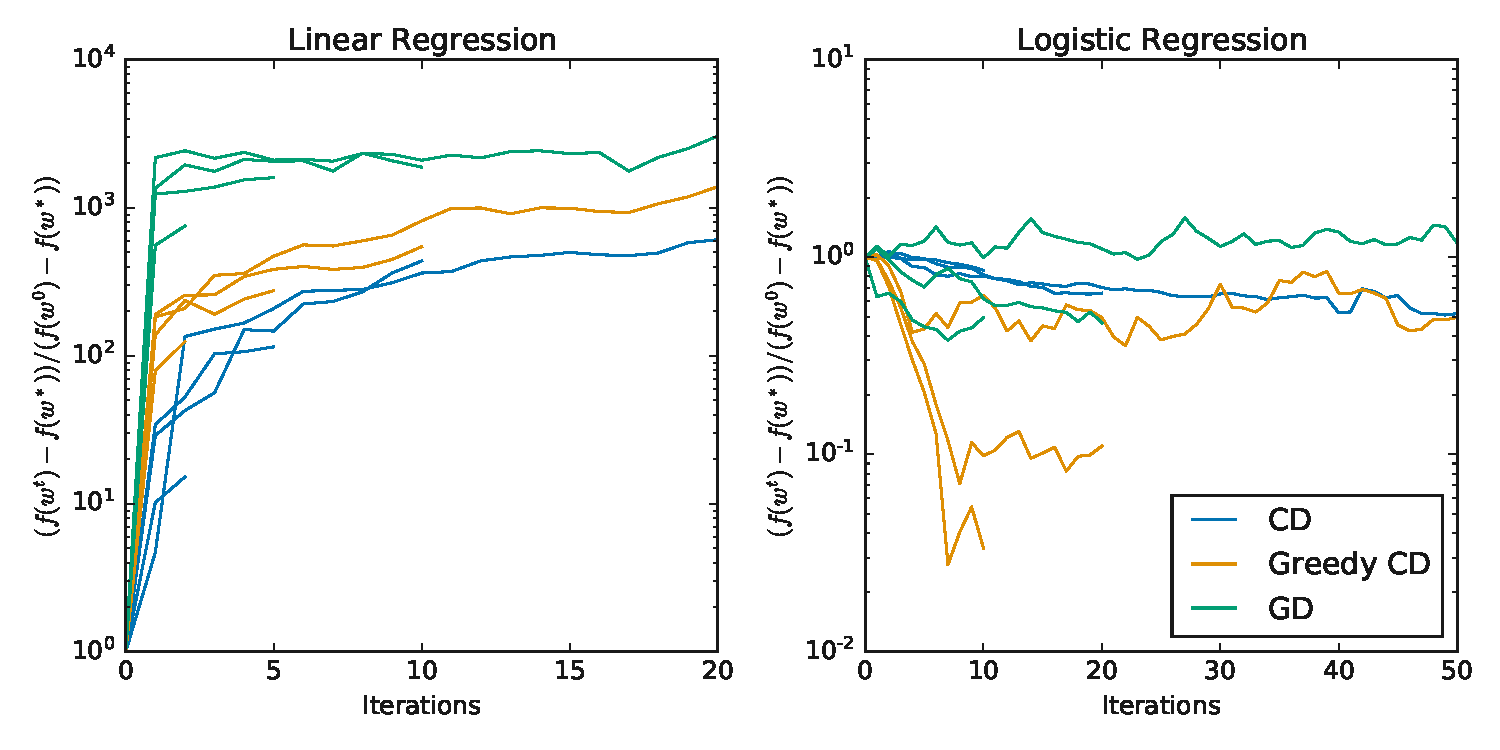
\includegraphics[width=1.0\linewidth]{images/cdvsgd_normal.pdf}
    \caption{Optimality gap for different number of iterations. Project iterates to $\ell_\infty$ ball of norm $50$. Mean of 5 runs. Note that iterations are iterations of algorithms and \textit{not} epochs.}
  \end{figure}
\end{frame}

\begin{frame}
  \begin{figure}
    \centering
    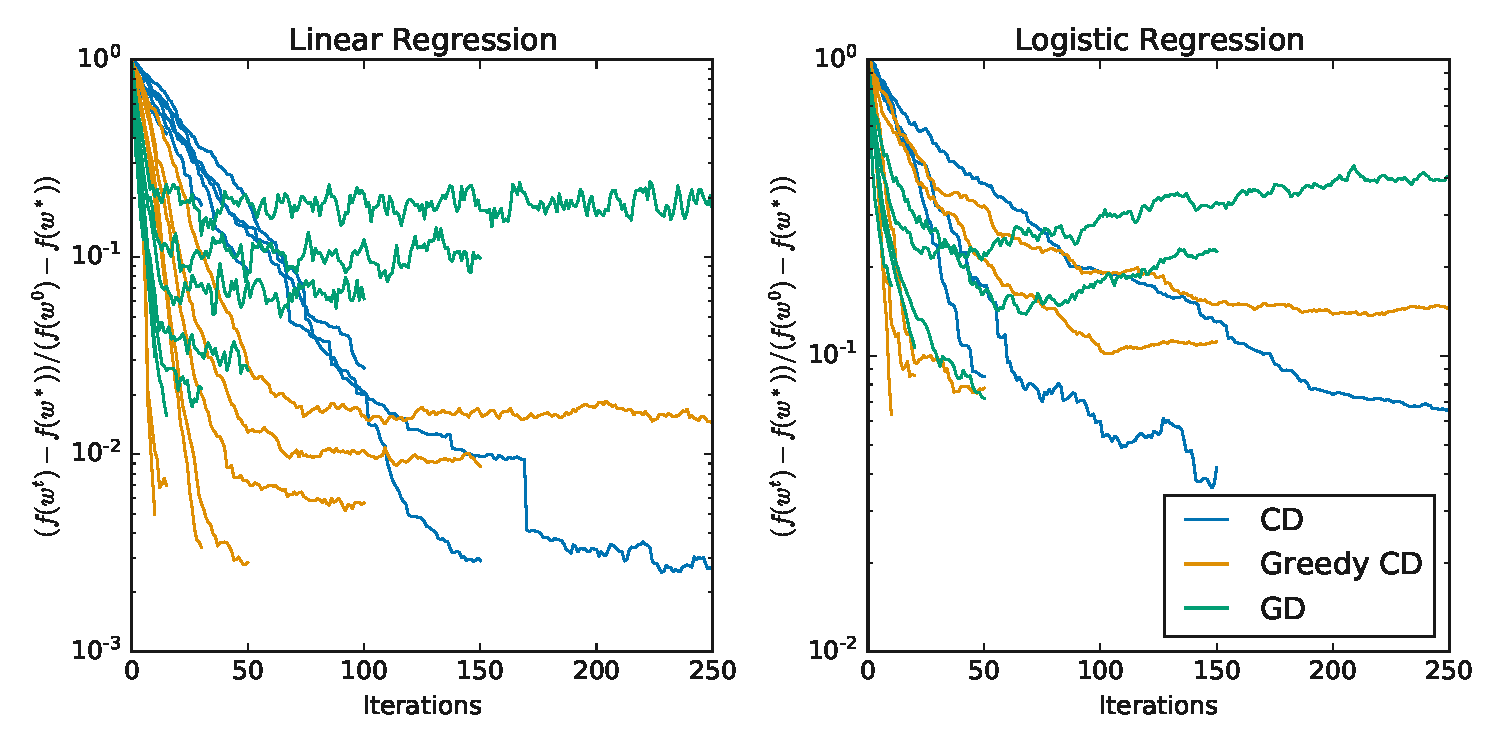
\includegraphics[width=1.0\linewidth]{images/cdvsgd_clipped.pdf}
    \caption{Optimality gap for different number of iterations. Clip Gradients (with tuned clipping). Mean of 5 runs. Note that iterations are iterations of algorithms and \textit{not} epochs.}
  \end{figure}
\end{frame}

\begin{frame}
  Comments:
  \begin{itemize}
  \item with clipping, a bound on iterates norms is not needed;
  \item without clipping, sensitivity is way too high: noise is too big to learn;
  \item on this example, DP-CD and DP-GD (with appropriate clipping) give similar (or better) utility.
  \end{itemize}
\end{frame}

\subsection{$\ell_1$ norm of rows set to $1$ - One Bigger Column}
\label{sub:l1_norm_of_rows_set_to1}


%%%%%%%%%%%%%%%%%%%%%%%%%%%%%%%%%%%%%%%%%%%%%%%%%%%%%%%%%%%%%%%%%%%%%%%%%%%%%%%%
\section{Conclusion}
\label{sec:conclusion}

\subsection{DP-ERM}
\label{sub:dp_erm}

\begin{frame}
  To sum up:
  \begin{itemize}
  \item ERM cannot be solved exactly under DP constraints;
  \item we know a lower bound on achievable utility;
  \item DP-SGD is nearly tight with respect to these lower bounds;
  \item restricting hypothesis class can lead to more precise results;
  \item in practice: difficult to get good utility while remaining DP.
  \end{itemize}
\end{frame}

\subsection{DP-CD for DP-ERM}
\label{sub:dp_cd_for_dp_erm}

\begin{frame}
  About DP-Coordinate Descent:
  \begin{itemize}
  \item DP-CD is theoretically not as good as DP-GD (or needs stronger hypotheses);
  \item in practice, it seems to achieve competitive convergence with appropriate clipping.
  \end{itemize}
\end{frame}

\begin{frame}
  Perspectives:
  \begin{itemize}
  \item analysis of clipping for CD (maybe easier than with GD?);
  \item tighter analysis of sum of coordinate-wise vs global sensitivities;
  \item DP-CD for composite functions;
  \item greedy variants also look promising.
  \end{itemize}
\end{frame}

\subsection{}

\begin{frame}
  Thank you for listening! :)
\end{frame}

\end{document}
%%% Local Variables:
%%% mode: latex
%%% TeX-master: t
%%% End:
